\documentclass[11pt]{amsart}

\date{\today}

\usepackage[margin=1in]{geometry}
\usepackage{tikz}
\usetikzlibrary{calc, shapes.geometric, positioning, shapes, snakes}
\usepackage{setspace}
\usepackage{amsmath}
\usepackage{amsthm}
\usepackage{amssymb}
\usepackage{mathtools}
\usepackage{mathdots}
\usepackage{enumitem}
\usepackage{graphicx}
\usepackage{caption}
\usepackage[labelformat=simple,labelfont={}]{subcaption}
\usepackage{color}
\definecolor{darkblue}{rgb}{0, 0, .6}
\usepackage{hyperref}
\hypersetup{
	colorlinks=true,
	linkcolor=darkblue,
	anchorcolor=darkblue,
	citecolor=darkblue,
	pagecolor=darkblue,
	urlcolor=darkblue,
	pdftitle=darkblue,
	pdfauthor=darkblue
}

\newtheorem{theorem}{Theorem}[subsection]
\newtheorem{lemma}[theorem]{Lemma}
\newtheorem{claim}[theorem]{Claim}
\newtheorem{corollary}[theorem]{Corollary}
\newtheorem{proposition}[theorem]{Proposition}
\newtheorem{conjecture}[theorem]{Conjecture}

\theoremstyle{definition} 
\newtheorem{definition}[theorem]{Definition}
\newtheorem{example}[theorem]{Example}
\newtheorem{remark}[theorem]{Remark}

\numberwithin{equation}{section}

\newcommand{\Z}{\mathbb{Z}}
\newcommand{\N}{\mathbb{N}}
\newcommand{\A}{\mathcal{A}}
\newcommand{\C}{\widetilde{C}}
\renewcommand{\O}{\mathcal{O}}
\newcommand{\E}{\mathcal{E}}
\newcommand{\z}{\mathsf{z}}
\newcommand{\x}{\mathsf{x}}
\newcommand{\y}{\mathsf{y}}
\renewcommand{\u}{\mathsf{u}}
\renewcommand{\v}{\mathsf{v}}
\newcommand{\wtri}{\vartriangle}
\newcommand{\btri}{\blacktriangle}
\renewcommand{\a}{\mathbf{a}}
\DeclareMathOperator{\TL}{TL}
\DeclareMathOperator{\DTL}{\mathbb{D}TL}
\renewcommand{\P}{\mathcal{P}}
\newcommand{\V}{\mathcal{V}}
\newcommand{\D}{\mathbb{D}}
\newcommand{\B}{\mathbf{B}}
\newcommand{\I}{\mathcal{I}}
\newcommand{\Diag}{\mathcal{D}}
\newcommand{\wcirc}{\circ}
\newcommand{\wbox}{\square}
\newcommand{\bcirc}{\bullet}
\newcommand{\bbox}{\blacksquare}
\newcommand{\supp}{\mathrm{supp}}
\renewcommand{\L}{\mathcal{L}}
\newcommand{\R}{\mathcal{R}}
\renewcommand{\(}{\left(}
\renewcommand{\)}{\right)}
\newcommand{\w}{\mathsf{w}}
\renewcommand{\H}{\mathcal{H}}
\DeclareMathOperator{\FC}{FC}
\renewcommand{\r}{\mathbf{r}}

\renewcommand\arraystretch{1.5}
\renewcommand\thesubfigure{(\alph{subfigure})}

%%% TikZ for Heaps %%%

%For Heaps. command of the form \heapblock{a}{b}{c} where a is the index of the generator, b is the level in the heap (starting at the bottom), c is the label

\newcommand\xxaxis{0}
\newcommand\yyaxis{90}

\newcommand\heapblock[3]{\fill[draw=black, fill=gray!30, rounded corners, line width=1.1pt, shift={(\xxaxis:#1)},shift={(\yyaxis:#2)}] (-1,-0.5) rectangle (1,0.5);\node at (#1,#2) {$#3$};}

\newcommand\heapblank[2]{\fill[fill=white, dotted, draw=black, line width=1.1pt, rounded corners, shift={(\xxaxis:#1)},shift={(\yyaxis:#2)}] (-1,-0.5) rectangle (1,0.5);}

%%% TikZ for Diagrams %%%

% loops
\newcommand\dlp[2]{
\fill[fill=white, draw=black] (#1,#2) ellipse (16pt and 8pt);
\draw[fill=black, xshift=-16pt] (#1,#2) circle (2.8pt);
}

\newcommand\lp[2]{\draw[out=90,in=90] (#1,#2) to (#1 + 1,#2) [out=-90,in=-90] to (#1,#2);}

\newcommand\blacktrilp[2]{\draw[out=90,in=90] (#1,#2) to node[blacktri, pos=0.5]{} (#1 + 1,#2) [out=-90,in=-90] to (#1,#2);}

\newcommand\whitetrilp[2]{\draw[out=90,in=90] (#1,#2) to node[whitetri, pos=0.5]{} (#1 + 1,#2) [out=-90,in=-90] to (#1,#2);}

\newcommand\blackwhitetrilp[2]{\draw[out=90,in=90] (#1,#2) to node[blacktri, pos=0.5]{} (#1 +1,#2) [out=-90,in=-90] to node[whitetri, pos=0.5]{} (#1,#2);}

%%%%%%%%%% begin document %%%%%%%%%%%

\begin{document}

\tikzstyle{blacktri} = [draw=black, fill=black, rotate=-90, sloped, regular polygon, regular polygon sides=3, inner sep=1.3pt]
\tikzstyle{whitetri} = [draw=black, fill=white, rotate=-90, sloped, regular polygon, regular polygon sides=3, inner sep=1.3pt]
\tikzstyle{blackcirc} = [draw=black, fill=black, shape=circle, inner sep=1.8pt]
\tikzstyle{whitecirc} = [draw=black, fill=white, shape=circle, inner sep=1.8pt]

\title[Diagram calculus for a type affine $C$ Temperley--Lieb algebra, II]{Diagram calculus for a type affine $C$ \\ Temperley--Lieb algebra, II}

\author[D.C.~Ernst]{Dana C.~Ernst}
\address{Department of Mathematics and Statistics, Northern Arizona University, Flagstaff, AZ 86011}
\email{\url{dana.ernst@nau.edu}}
\urladdr{\url{http://danaernst.com}}

\subjclass[2000]{20F55, 20C08, 57M15}
\keywords{diagram algebra, Temperley--Lieb algebra, Coxeter groups, heaps}

%%%%%%%%%% abstract %%%%%%%%%%%

\begin{abstract}
In a previous paper, we presented an infinite dimensional associative diagram algebra that satisfies the relations of the generalized Temperley--Lieb algebra having a basis indexed by the fully commutative elements (in the sense of Stembridge) of the Coxeter group of type affine $C$.  We also provided an explicit description of a basis for the diagram algebra.  In this paper, we show that this diagrammatic representation is faithful.
\end{abstract}

\maketitle

{\color{red}Be sure to fix reference to ``where the rectangle" in figures such as \ref{fig:western C5}. Actually, check all references to diagrams with $\mathbf{b}$.}

%%%%%%%  introduction %%%%%%%%%%%%%

\begin{section}{Introduction}\label{sec:intro}

The (type $A$) Temperley--Lieb algebra $\TL(A)$, invented by H.N.V.~Temperley and E.H.~Lieb in 1971~\cite{Temperley1971}, is a finite dimensional associative algebra which first arose in the context of statistical mechanics.  R.~Penrose and L.H.~Kauffman showed that this algebra can be realized as a diagram algebra having a basis given by certain diagrams in which the multiplication rule is given by applying local combinatorial rules to the diagrams~\cite{Kauffman1987, Penrose1971}.

In 1987, V.F.R.~Jones showed that $\TL(A)$ occurs naturally as a quotient of the type $A$ Hecke algebra, $\H(A)$~\cite{Jones1999}.  If $(W,S)$ is Coxeter system of type $\Gamma$, the associated Hecke algebra $\H(\Gamma)$ is an algebra with a basis given by $\{T_w\mid w \in W\}$ and relations that deform the relations of $W$ by a parameter $q$. The realization of the Temperley--Lieb algebra as a Hecke algebra quotient was generalized by J.J.~Graham in~\cite{Graham1995} to the case of an arbitrary Coxeter system.  In Section~\ref{subsec:TL-algebras}, we define the generalized Temperley--Lieb algebra of type $\C_{n}$, denoted $\TL(\C_{n})$, and describe a special basis, called the monomial basis, which is indexed by the fully commutative elements (defined in Section~\ref{subsec:FC}) of the underlying Coxeter group.

The goal of this paper is to establish a faithful diagrammatic representation of the Tem\-per\-ley--Lieb algebra (in the sense of Graham) of type $\C$.  One motivation behind this is that a realization of $\TL(\C_n)$ can be of great value when it comes to understanding the otherwise purely abstract algebraic structure of the algebra.  Moreover, studying these generalized Temperley--Lieb algebras often provides a gateway to understanding the Kazhdan--Lusztig theory of the associated Hecke algebra.  Loosely speaking, $\TL(\Gamma)$ retains some of the relevant structure of $\H(\Gamma)$, yet is small enough that computation of the leading coefficients of the notoriously difficult to compute Kazhdan--Lusztig polynomials is often much simpler.

In~\cite{Ernst2012}, we constructed an infinite dimensional associative diagram algebra $\D_n$.  We were able to easily check that this algebra satisfies the relations of $\TL(\C_n)$, thus showing that there is a surjective algebra homomorphism from $\TL(\C_n)$ to $\D_n$.  Moreover, we described the set of admissible diagrams by providing a combinatorial description of the allowable edge configurations involving diagram decorations (Definition~\ref{def:admissible} in this paper), and we accomplished the more difficult task of proving that this set of diagrams forms a basis for $\D_n$.  However, due to length considerations, it remained to be shown that our diagrammatic representation is faithful and that each admissible diagram corresponds to a unique monomial basis element of $\TL(\C_n)$.  The main result of this paper (Theorem~\ref{thm:main result}) establishes the faithfulness of our diagrammatic representation and the correspondence between the admissible diagrams and the monomial basis elements of $\TL(\C_n)$.

With the exception of type $\widetilde{A}$, all other generalized Temperley--Lieb algebras with known diagrammatic representations are finite dimensional.  In the finite dimensional case, counting arguments are employed to prove faithfulness, but these techniques are not available in the type $\C$ case since $\TL(\C_n)$ is infinite dimensional.  Instead, we will make use of the author's classification in~\cite{Ernst2010} of the non-cancellable elements in Coxeter groups of types $B$ and $\C$ (Propositions~\ref{prop:Bwsrm} and~\ref{prop:affineCwsrm} in this paper).  The classification of the non-cancellable elements in Coxeter groups of type $\C$ provides the foundation for inductive arguments used to prove the faithfulness of $\D_n$.  The diagram algebra $\D_n$ presented here and in~\cite{Ernst2012} is the first faithful representation of an infinite dimensional non-simply-laced generalized Temperley--Lieb algebra (in the sense of Graham).

Section~\ref{sec:prelim} of this paper is concerned with introducing the necessary notation and terminology of Coxeter groups, fully commutative elements, and heaps.  The concept of a heap introduced in Section~\ref{subsec:heaps} will be our main tool for visualizing combinatorial arguments required to prove several technical lemmas appearing in Section~\ref{subsec:prep lemmas}.  In Section~\ref{sec:combinatorics}, we study some of the combinatorics of Coxeter groups of types $B$ and $\C$.  In particular, we introduce weak star reductions and the type I, type II, and non-cancellable elements of a Coxeter group of type $\C$, as well as establish several intermediate results.  The necessary background on generalized Temperley--Lieb algebras (in the sense of Graham) is summarized in Section~\ref{sec:gen TL-algebras}.  The goal of Section~\ref{sec:diagram algebras} is to familiarize the reader with the conventions and terminology of diagram algebras necessary to define the diagram algebra $\D_n$ and to describe the admissible diagrams.  Our main result (Theorem~\ref{thm:main result}), which establishes the faithful diagrammatic representation of $\TL(\C_n)$ by $\D_n$, finally comes in Section~\ref{subsec:injectivity} after proving a few additional lemmas in Sections~\ref{subsec:hom} and \ref{subsec:additional prep lemmas}.  Lastly, in Section~\ref{sec:closing}, we discuss the implications of our results and future research.

\end{section}

%%%%%%%  preliminaries %%%%%%%%%%%%%

\begin{section}{Preliminaries}\label{sec:prelim}

%%%%%%%%%%%%% Coxeter groups %%%%%%%%%%%%

\begin{subsection}{Coxeter groups}\label{subsec:coxeter groups}

A \emph{Coxeter system} is pair $(W,S)$ consisting of a distinguished (finite) set $S$ of generating involutions and a group $W$, called a \emph{Coxeter group}, with presentation
\[
W = \langle S \mid (st)^{m(s, t)} = e \text{ for } m(s, t) < \infty \rangle,
\]
where $e$ is the identity, $m(s,t) = 1$ if and only if $s = t$, and $m(s,t) = m(t,s)$. It turns out that the elements of $S$ are distinct as group elements, and that $m(s, t)$ is the order of $st$.  Since the elements of $S$ have order two, the relation $(st)^{m(s,t)} = e$ can be written as
\[
\underbrace{sts \cdots}_{m(s,t)} = \underbrace{tst \cdots}_{m(s,t)}
\]
with $m(s,t) \geq 2$ factors.

Given a Coxeter system $(W,S)$, a word $s_{x_1}s_{x_2}\cdots s_{x_m}$ in the free monoid $S^*$ is called an \emph{expression} for $w\in W$ if it is equal to $w$ when considered as a group element. If $m$ is minimal among all expressions for $w$, the corresponding word is called a \emph{reduced expression} for $w$. In this case, we define the \emph{length} of $w$ to be $\ell(w)=m$. Each element $w \in W$ can have several different reduced expressions that represent it.  If we wish to emphasize a fixed, possibly reduced, expression for $w\in W$, we represent it  in \textsf{sans serif} font, say $\w=s_{x_1}s_{x_2}\cdots s_{x_m}$, where each $s_{x_i} \in S$.  A product $w_{1}w_{2}\cdots w_{r}$ with $w_{i} \in W$ is called \emph{reduced} if $\ell(w_{1}w_{2}\cdots w_{r})=\sum \ell(w_{i})$.  

Matsumoto's Theorem~\cite[Theorem 1.2.2]{Geck2000} states that if $w \in W$, then every reduced expression for $w$ can be obtained from any other by applying a sequence of \emph{braid moves} of the form 
\[
{\underbrace{sts \cdots }_{m(s,t)} } \mapsto {\underbrace{tst \cdots}_{m(s,t)}}
\]
where $s,t \in S$ and each factor in the move has $m(s,t)$ letters.  The \emph{support} of an element $w \in W$, denoted $\supp(w)$, is the set of all generators appearing in any reduced expression for $w$ (which is well-defined by Matsumoto's Theorem).

Given a reduced expression $\w$ for $w \in W$, we define a \emph{subexpression} of $\w$ to be any subsequence of $\w$. We will refer to a subexpression consisting of a string of consecutive symbols from $\w$ as a \emph{subword} of $\w$.

The sets $\L(w)=\{s \in S\mid \ell(sw) < \ell(w)\}$ and $\R(w)=\{s \in S\mid \ell(ws) < \ell(w)\}$ are called the \emph{left} and \emph{right descent sets} of $w$, respectively.  It turns out that $s \in \L(w)$ (respectively, $\R(w)$) if and only if $w$ has a reduced expression beginning (respectively, ending) with $s$.

Given a Coxeter system $(W,S)$, the associated \emph{Coxeter graph} is the graph $\Gamma$ with vertex set $S$ and edges $\{s,t\}$ labeled with $m(s,t)$ for all $m(s,t)\geq 3$.  If $m(s,t)=3$, it is customary to leave the corresponding edge unlabeled.  Given a Coxeter graph $\Gamma$, we can uniquely reconstruct the corresponding Coxeter system $(W,S)$.  In this case, we say that $(W,S)$, or just $W$, is of type $\Gamma$. If $(W,S)$ is of type $\Gamma$, for emphasis, we may write $(W,S)$ as $(W(\Gamma),S(\Gamma))$.  Note that generators $s$ and $t$ are connected by an edge in the Coxeter graph $\Gamma$ if and only if $s$ and $s$ do not commute \cite{Humphreys1990}.

The main focus of this paper will be the Coxeter systems of types $B_n$ and $\C_n$, which are defined by the Coxeter graphs in Figures \ref{typeB} and \ref{typeC}, respectively, where $n\geq 2$.

\begin{figure}[!ht]
\subcaptionbox{Type $B_n$\label{typeB}}[.4\textwidth]{
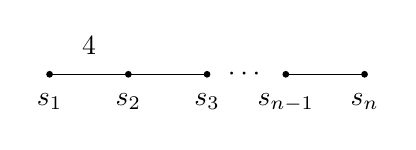
\begin{tikzpicture}
\draw[fill=black] \foreach \x in {1,2,3,4,5} {(\x,10) circle (1pt)};
\draw \foreach \x in {1,2,3} {(\x,10) node[label=below:$s_{\x}$]{}};
\draw (1.5,10) node[label=above:$4$]{};
\draw {(4,10) node[label=below:$s_{n-1}$]{}};
\draw {(5,10) node[label=below:$s_{n}$]{}};
\draw {(3.5,10) node[]{$\cdots$}};
\draw[-] (1,10) -- (3,10);
\draw[-] (4,10) -- (5,10);
\end{tikzpicture}
}
\subcaptionbox{Type $\C_n$\label{typeC}}[.4\textwidth]{
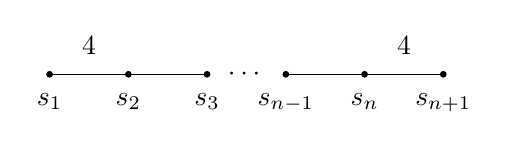
\begin{tikzpicture}
\draw[fill=black] \foreach \x in {1,2,3,4,5,6} {(\x,10) circle (1pt)};
\draw \foreach \x in {1,2,3} {(\x,10) node[label=below:$s_{\x}$]{}};
\draw (1.5,10) node[label=above:$4$]{};
\draw {(4,10) node[label=below:$s_{n-1}$]{}};
\draw {(5,10) node[label=below:$s_{n}$]{}};
\draw {(6,10) node[label=below:$s_{n+1}$]{}};
\draw {(3.5,10) node[]{$\cdots$}};
\draw (5.5,10) node[label=above:$4$]{};
\draw[-] (1,10) -- (3,10);
\draw[-] (4,10) -- (6,10);
\end{tikzpicture}
}
\caption{Coxeter graphs corresponding to Coxeter systems of type $A_{n}$ and $D_{n}$.}
\end{figure}

We can obtain $W(B_{n})$ from $W(\C_{n})$ by removing the generator $s_{n+1}$ and the corresponding relations~\cite[Chapter 5]{Humphreys1990}.  We also obtain a Coxeter group of type $B$ if we remove the generator $s_{1}$ and the corresponding relations.  To distinguish these two cases, we let $W(B_{n})$ denote the subgroup of $W(\C_{n})$ generated by $\{s_{1}, s_{2}, \dots, s_{n}\}$ and we let $W(B'_{n})$ denote the subgroup of $W(\C_{n})$ generated by $\{s_{2}, s_{3}, \dots, s_{n+1}\}$.  It is well known that $W(\C_{n})$ is an infinite Coxeter group while $W(B_{n})$ and $W(B'_{n})$ are both finite~\cite[Chapters 2 and 6]{Humphreys1990}.

\end{subsection}

%%%%%%%%  FC elements %%%%%%%%%%%%%

\begin{subsection}{Fully commutative elements}\label{subsec:FC}

Let $(W,S)$ be a Coxeter system of type $\Gamma$ and let $w \in W$. Following Stembridge~\cite{Stembridge1996}, we define a relation $\sim$ on the set of reduced expressions for $w$.  Let $\w$ and $\w'$ be two reduced expressions for $w$.  We define $\w \sim \w'$ if we can obtain $\w'$ from $\w$ by applying a single commutation move of the form $st \mapsto ts$, where $m(s,t)=2$.  Now, define the equivalence relation $\approx$ by taking the reflexive transitive closure of $\sim$.  Each equivalence class under $\approx$ is called a \emph{commutation class}. If $w$ has a single commutation class, then we say that $w$ is \emph{fully commutative} (FC).  According to a result in~\cite{Stembridge1996}, an element $w$ is FC if and only if no reduced expression for $w$ contains a subword of the form $sts \cdots$ of length $m(s,t) \geq 3$.  The set of FC elements of the Coxeter system $(W,S)$ of type $\Gamma$ is denoted by $\FC(\Gamma)$, or possibly $\FC(W)$.

\begin{remark}\label{rem:illegal convex chains}
The elements of $\FC(\C_{n})$ are precisely those whose reduced expressions avoid consecutive subwords of the following types:
\begin{enumerate}
\item $s_{i}s_{j}s_{i}$ for $|i-j|=1$ and $1< i,j < n+1$;
\item $s_{i}s_{j}s_{i}s_{j}$ for $\{i,j\}=\{1,2\}$ or $\{n,n+1\}$.
\end{enumerate}
Note that the FC elements of $W(B_{n})$ and $W(B'_{n})$ avoid the respective subwords above.
\end{remark}

In~\cite{Stembridge1996}, Stembridge classified the Coxeter groups that contain a finite number of FC elements.  According to~\cite[Theorem 5.1]{Stembridge1996}, $W(\C_{n})$ contains an infinite number of FC elements, while $W(B_{n})$ (and hence $W(B'_n)$) contains finitely many.  There are examples of infinite Coxeter groups that contain a finite number of FC elements (e.g., $W(E_n$) is infinite for $n\geq 9$, but contains only finitely many FC elements~\cite[Theorem 5.1]{Stembridge1996}).

\end{subsection}

%%%%%%%%%%%%%%%%%%%%%

\begin{subsection}{Heaps}\label{subsec:heaps}

Every reduced expression can be associated with a partially ordered set called a heap that will allow us to visualize a reduced expression  while preserving the essential information about the relations among the generators.  The theory of heaps was introduced in~\cite{Viennot1986} by Viennot and visually capture the combinatorial structure of the Cartier--Foata monoid of~\cite{Cartier1969}.  In~\cite{Stembridge1996} and~\cite{Stembridge1998}, Stembridge studied heaps in the context of FC elements, which is our motivation here.  In this section, we mimic the development found in~\cite{Billey2007},~\cite{Ernst2010}, and~\cite{Stembridge1996}.

Let $(W,S)$ be a Coxeter system.  Suppose $\w = s_{x_1} \cdots s_{x_r}$ is a fixed reduced expression for $w \in W$.  As in~\cite{Stembridge1996}, we define a partial ordering on the indices $\{1, \dots, r\}$ by the transitive closure of the relation $\lessdot$ defined via $j \lessdot i$ if $i < j$ and $s_{x_i}$ and $s_{x_j}$ do not commute.  In particular, since $\w$ is reduced, $j \lessdot i$ if $i < j$ and $s_{x_i} = s_{x_j}$ by transitivity.  This partial order is referred to as the \emph{heap} of $\w$, where $i$ is labeled by $s_{x_i}$  Note that for simplicity, we are omitting the labels of the underlying poset but retaining the labels of the corresponding generators.

It follows from~\cite[Proposition 2.2]{Stembridge1996} that heaps are well-defined up to commutativity class.  That is, if $\w$ and $\w'$ are two reduced expressions for $w \in W$ that are in the same commutativity class, then the heaps of $\w$ and $\w'$ are equal.  In particular, if $w$ is FC, then it has a single commutativity class, and so there is a unique heap associated to $w$.

\begin{example}\label{ex:first heap}
Let $\w = s_3 s_2 s_1 s_2 s_5s_{4}s_{6}s_{5}$ be a reduced expression for $w \in \FC(\C_{5})$.  We see that $\w$ is indexed by $\{1, 2, 3, 4, 5, 6, 7, 8\}$.  As an example, $3 \lessdot 2$ since $2 < 3$ and the second and third generators do not commute.  The labeled Hasse diagram for the heap poset of $w$ is shown in Figure~\ref{fig:hasse}.
\end{example}

\begin{figure}[!ht]
\subcaptionbox{\label{fig:hasse}}[.4\textwidth]{ 
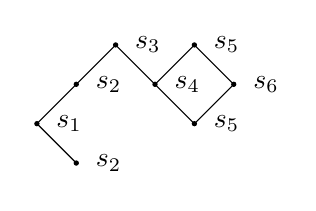
\begin{tikzpicture}[scale=0.5]
\draw [fill=black] (2,1) circle (1.5pt);
\draw (2,1) node[label=right:$s_2$]{};
\draw [fill=black] (1,2) circle (1.5pt);
\draw (1,2) node[label=right:$s_1$]{};
\draw [fill=black] (5,2) circle (1.5pt);
\draw (5,2) node[label=right:$s_5$]{};
\draw [fill=black] (2,3) circle (1.5pt);
\draw (2,3) node[label=right:$s_2$]{};
\draw [fill=black] (4,3) circle (1.5pt);
\draw (4,3) node[label=right:$s_4$]{};
\draw [fill=black] (6,3) circle (1.5pt);
\draw (6,3) node[label=right:$s_6$]{};
\draw [fill=black] (3,4) circle (1.5pt);
\draw (3,4) node[label=right:$s_3$]{};
\draw [fill=black] (5,4) circle (1.5pt);
\draw (5,4) node[label=right:$s_5$]{};
\draw [color=white] (1,.5) circle (0pt);
\draw (2,1)--(1,2)--(2,3)--(3,4)--(4,3)--(5,2)--(6,3)--(5,4)--(4,3);
\end{tikzpicture}
}
\subcaptionbox{\label{fig:first heap}}[.4\textwidth]{
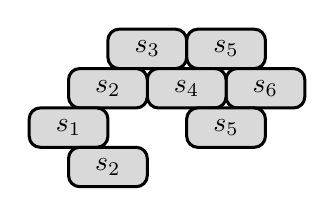
\begin{tikzpicture}[scale=0.5]
\heapblock{5}{4}{s_5};
\heapblock{3}{4}{s_3};
\heapblock{6}{3}{s_6};
\heapblock{4}{3}{s_4};
\heapblock{2}{3}{s_2};
\heapblock{5}{2}{s_5};
\heapblock{1}{2}{s_1};
\heapblock{2}{1}{s_2};
\end{tikzpicture}
}
\caption{The labeled Hasse diagram and a possible lattice point representation for the heap of an element from $\FC(\C_5)$.}
\end{figure}

Let $\w$ be a fixed reduced expression for $w \in W(\C_{n})$.  As in~\cite{Billey2007} and~\cite{Ernst2010}, we will represent a heap for $\w$ as a set of lattice points embedded in $\{1,2,\ldots,n+1\} \times \mathbb{N}$.  To do so, we assign coordinates (not unique) $(x,y) \in \{1,2,\ldots, n+1\} \times \mathbb{N}$ to each entry of the labeled Hasse diagram for the heap of $\w$ in such a way that:
\begin{enumerate}
\item an entry with coordinates $(x,y)$ is labeled $s_i$ in the heap if and only if $x = i$; 
\item an entry with coordinates $(x,y)$ is greater than an entry with coordinates $(x',y')$ in the heap if and only if $y > y'$.
\end{enumerate}

Recall that a finite poset is determined by its covering relations.  In the case of a Coxeter group of type $\C_{n}$ (and any straight line Coxeter graph), it follows from the definition that $(x,y)$ covers $(x',y')$ in the heap if and only if $x = x' \pm 1$, $y > y'$, and there are no entries $(x'', y'')$ such that $x'' \in \{x, x'\}$ and $y'< y'' < y$.  This implies that we can completely reconstruct the edges of the Hasse diagram and the corresponding fig:heap poset from a lattice point representation. The lattice point representation of a heap allows us to visualize potentially cumbersome arguments.  As in~\cite{Ernst2010}, our heaps are upside-down versions of the heaps that appear in~\cite{Billey2007} and several other papers.  That is, in this paper entries at top of a heap correspond to generators occurring to the left, as opposed to the right, in the corresponding reduced expression.  Our convention aligns more naturally with the typical conventions of diagram algebras.

Let $\w$ be a reduced expression for $w \in W(\C_{n})$.  We let $H(\w)$ denote a lattice representation of the heap poset in $\{1,2,\ldots,n+1\} \times \N$ described in the preceding paragraphs.  If $w$ is FC, then the choice of reduced expression for $w$ is irrelevant, in which case, we will often write $H(w)$ (note the absence of \textsf{sans serif} font) and we will refer to $H(w)$ as the heap of $w$.

Given a heap, there are many possible coordinate assignments, yet the $x$-coordinates for each entry will be fixed for all of them.  In particular, two entries labeled by the same generator may only differ by the amount of vertical space between them while maintaining their relative vertical position to adjacent entries in the heap.

Let $\w=s_{x_1}\cdots s_{x_r}$ be a reduced expression for $w \in \FC(\C_{n})$.  If $s_{x_i}$ and $s_{x_j}$ are adjacent generators in the Coxeter graph with $i<j$, then we must place the point labeled by $s_{x_i}$ at a level that is \emph{above} the level of the point labeled by $s_{x_j}$.  Because generators that are not adjacent in the Coxeter graph do commute, points whose $x$-coordinates differ by more than one can slide past each other or land at the same level.  To emphasize the covering relations of the lattice representation we will enclose each entry of the heap in a rectangle in such a way that if one entry covers another, the rectangles overlap halfway.

\begin{example}\label{ex:second heap}
Let $w$ be as in Example~\ref{ex:first heap}.  Then one possible representation for $H(w)$ appears in Figure~\ref{fig:first heap}.
\end{example}

When $w$ is FC, we wish to make a canonical choice for the representation $H(w)$ by assembling the entries in a particular way.  To do this, we give all entries corresponding to elements in $\L(w)$ the same vertical position and all other entries in the heap should have vertical position as high as possible.  For example, the representation of $H(w)$ given in Figure~\ref{fig:first heap} is the canonical representation.  Note that our canonical representation of heaps of FC elements corresponds precisely to the unique heap factorization of~\cite[Lemma 2.9]{Viennot1986} and to the Cartier--Foata normal form for monomials~\cite{Cartier1969,Green2006a}.  When illustrating heaps, we will adhere to this canonical choice, and when we consider the heaps of arbitrary reduced expressions, we will only allude to the relative vertical positions of the entries, and never their absolute coordinates.  

Let $w \in \FC(\C_n)$ have reduced expression $\w=s_{x_1}\cdots s_{x_r}$ and suppose $s_{x_i}$ and $s_{x_j}$ equal the same generator $s_k$, so that the corresponding entries have $x$-coordinate $k$ in $H(w)$.  We say that $s_{x_i}$ and $s_{x_j}$ are \emph{consecutive} if there is no other occurrence of $s_{k}$ occurring between them in $\w$.

Let $\w=s_{x_{1}} \cdots s_{x_{r}}$ be a reduced expression for $w \in W(\C_{n})$.  We define a heap $H'$ to be a \emph{subheap} of $H(\w)$ if $H'=H(\w')$, where $\w'=s_{y_1}s_{y_2} \cdots s_{y_k}$ is a subexpression of $\w$.  We emphasize that the subexpression need not be a subword (i.e., a consecutive subexpression).

A subheap $H'$ of $H(\w)$ is called a \emph{saturated subheap} if whenever $s_{i}$ and $s_{j}$ occur in $H'$ such that there exists a saturated chain from $i$ to $j$ in the underlying poset for $H(\w)$, there also exists a saturated chain $i=i_{k_{1}}<i_{k_{2}}< \cdots < i_{k_{l}}=j$ in the underlying poset for $H'$ such that the same chain is also a saturated chain in the underlying poset for $H(\w)$.

Recall that a subposet $Q$ of $P$ is called convex if $y \in Q$ whenever $x < y < z$ in $P$ and $x, z \in Q$.  A \emph{convex subheap} is a subheap in which the underlying subposet is convex.

\begin{example}\label{ex:third heap}
Let $\w= s_3 s_2 s_1 s_2 s_5s_{4}s_{6}s_{5}$ as in Example~\ref{ex:first heap}.  Also, let $\w'=s_3 s_1 s_{5}$ be the subexpression of $\w$ that results from deleting all but the first, third, and last generators of $\w$.  Then $H(\w')$ is equal to the heap in Figure~\ref{fig:subheap} and is a subheap of $H(\w)$.  However, $H(\w')$ is neither a saturated or a convex subheap of $H(\w)$ since there is a saturated chain in $H(\w)$ from the lower occurrence of $s_{5}$ to the occurrence of $s_{3}$, but there is not a chain between the corresponding entries in $H(\w')$.  Now, let $\w''=s_{5}s_{4}s_{5}$ be the subexpression of $\w$ that results from deleting all but the fifth, sixth, and last generators of $\w$.  Then $H(\w'')$ equals the heap in Figure~\ref{fig:convex subheap} and is a saturated subheap of $H(\w)$, but it is not a convex subheap since there is an entry in $H(\w)$ labeled by $s_{6}$ occurring between the two consecutive occurrences of $s_{5}$ that does not occur in $H(\w'')$.  However, if we do include the entry labeled by $s_{6}$, then the heap in Figure~\ref{fig:saturated subheap}  is a convex subheap of $H(\w)$.  
\end{example}

\begin{figure}[!ht]
\subcaptionbox{\label{fig:subheap}}[.3\textwidth]{
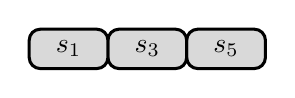
\begin{tikzpicture}[scale=0.5]
\heapblock{5}{1}{s_5};
\heapblock{3}{1}{s_3};
\heapblock{1}{1}{s_1};
\end{tikzpicture}
}
\subcaptionbox{\label{fig:convex subheap}}[.3\textwidth]{
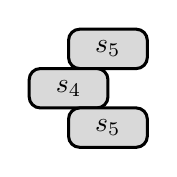
\begin{tikzpicture}[scale=0.5]
\heapblock{5}{3}{s_5};
\heapblock{4}{2}{s_4};
\heapblock{5}{1}{s_5};
\end{tikzpicture}
}
\subcaptionbox{\label{fig:saturated subheap}}[.3\textwidth]{
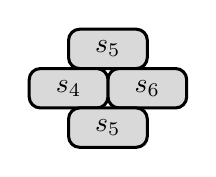
\begin{tikzpicture}[scale=0.5]
\heapblock{5}{3}{s_5};
\heapblock{6}{2}{s_6};
\heapblock{4}{2}{s_4};
\heapblock{5}{1}{s_5};
\end{tikzpicture}
}
\caption{Various subheaps of the heap in given in Figure~\ref{fig:first heap}.}
\label{fig:subheaps}
\end{figure}

From this point on, if there can be no confusion, we will not specify the exact subexpression that a subheap arises from.

The following fact is implicit in the literature (in particular, see the proof of~\cite[Proposition 3.3]{Stembridge1996}) and follows easily from the definitions.

\begin{proposition}
Let $(W,S)$ be a Coxeter system of type $\Gamma$ and let $w \in \FC(\Gamma)$. Then $H'$ is a convex subheap of $H(w)$ if and only if $H'$ is the heap for some subword of some reduced expression for $w$.   \qed
\end{proposition}

It will be extremely useful for us to be able to recognize when a heap corresponds to an element in $\FC(\C_{n})$.  The following lemma follows immediately from Remark~\ref{rem:illegal convex chains} and is also a special case of~\cite[Proposition 3.3]{Stembridge1996}.

\begin{lemma}\label{lem:impermissible heap configs}
Let $w \in \FC(\C_{n})$.  Then $H(w)$ cannot contain any of the following convex subheaps of Figure~\ref{fig:impermissible heap configs}, where $1<k<n+1$ and we use \begin{tabular}{c} 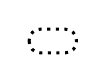
\begin{tikzpicture}[scale=0.3] \heapblank{0}{0}; \end{tikzpicture} \end{tabular} to emphasize that no element of the heap occupies the corresponding position.  \qed
\end{lemma}

\begin{figure}[!ht]
\subcaptionbox{}[.3\linewidth]{
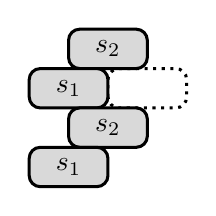
\begin{tikzpicture}[scale=0.5]
\heapblank{3}{3}
\heapblock{2}{4}{s_2};
\heapblock{1}{3}{s_1};
\heapblock{2}{2}{s_2};
\heapblock{1}{1}{s_1};
\end{tikzpicture}
}
\subcaptionbox{}[.3\linewidth]{
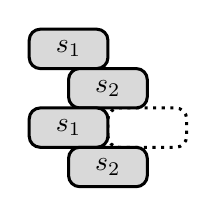
\begin{tikzpicture}[scale=0.5]
\heapblank{3}{2}
\heapblock{1}{4}{s_1};
\heapblock{2}{3}{s_2};
\heapblock{1}{2}{s_1};
\heapblock{2}{1}{s_2};
\end{tikzpicture}
}
\subcaptionbox{}[.3\linewidth]{
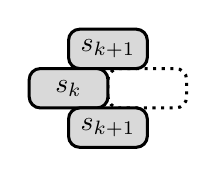
\begin{tikzpicture}[scale=0.5]
\heapblank{3}{2}
\heapblock{2}{3}{s_{k+1}};
\heapblock{1}{2}{s_k};
\heapblock{2}{1}{s_{k+1}};
\end{tikzpicture}
}\\
\vspace{1em}
\subcaptionbox{}[.3\linewidth]{
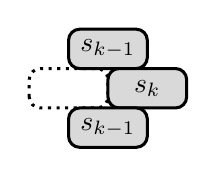
\begin{tikzpicture}[scale=0.5]
\heapblank{0}{2}
\heapblock{1}{3}{s_{k-1}};
\heapblock{2}{2}{s_k};
\heapblock{1}{1}{s_{k-1}};
\end{tikzpicture}
}
\subcaptionbox{}[.3\linewidth]{
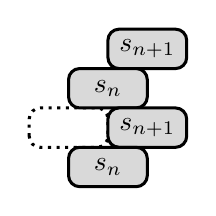
\begin{tikzpicture}[scale=0.5]
\heapblank{0}{2}
\heapblock{2}{4}{s_{n+1}};
\heapblock{1}{3}{s_n};
\heapblock{2}{2}{s_{n+1}};
\heapblock{1}{1}{s_n};
\end{tikzpicture}
}
\subcaptionbox{}[.3\linewidth]{
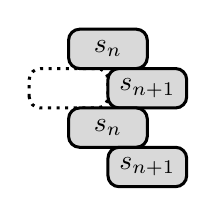
\begin{tikzpicture}[scale=0.5]
\heapblank{0}{3}
\heapblock{1}{4}{s_n};
\heapblock{2}{3}{s_{n+1}};
\heapblock{1}{2}{s_n};
\heapblock{2}{1}{s_{n+1}};
\end{tikzpicture}
}
\caption{Impermissible convex subheaps for elements in $\FC(\C_n)$.}\label{fig:impermissible heap configs}
\end{figure}

\end{subsection}

\end{section}

%%%%%%%%%%  Combinatorics in Coxeter groups of type affine $C$ %%%%%%%%%%%%%

\begin{section}{Combinatorics in Coxeter groups of type affine $C$}\label{sec:combinatorics}

In this section, we explore some of the relevant combinatorics in Coxeter groups of type $\C$.

%%%%%%%%%%  type I and type II elements %%%%%%%%%%%%%

\begin{subsection}{Type I and type II elements}

Let $w \in \FC(\C_{n})$.  We define $n(w)$ to be the maximum integer $k$ such that $w$ has a reduced expression of the form $w = u x v$ (reduced), where $u, x, v \in \FC(\C_{n})$, $\ell(x)=k$, and $x$ is a product of commuting generators.  Note that $n(w)$ may be greater than the size of any row in the canonical representation of $H(w)$.  It is known that $n(w)$ is equal to the size of a maximal antichain in the fig:heap poset for $w$~\cite[Lemma 2.9]{Shi2005}.

\begin{definition}\label{def:zigzags}
Define the following elements of $W(\C_{n})$.
\begin{enumerate}
\item If $i<j$, let
\[
\z_{i,j}=s_{i}s_{i+1}\cdots s_{j-1}s_{j}
\]
and
\[
\z_{j,i}=s_{j}s_{j-1}\cdots s_{i-1}s_{i}.
\]
We also let $\z_{i,i}=s_{i}$.

\item If $1< i \leq n+1$ and $1 < j \leq n+1$, let
\[
\z^{L,2k}_{i,j}=\z_{i,2}(\z_{1,n}\z_{n+1,2})^{k-1}\z_{1,n}\z_{n+1,j}.
\]
\item If $1< i \leq n+1$ and $1 \leq j < n+1$, let
\[
\z^{L,2k+1}_{i,j}=\z_{i,2}(\z_{1,n}\z_{n+1,2})^{k}\z_{1,j}.
\]

\item If $1\leq i < n+1$ and $1 \leq j <  n+1$, let
\[
\z^{R,2k}_{i,j}=\z_{i,n}(\z_{n+1,2}\z_{1,n})^{k-1}\z_{n+1,2}\z_{1,j}.
\]
	
\item If $1\leq i < n+1$ and $1 < j \leq  n+1$, let 
\[
\z^{R,2k+1}_{i,j}=\z_{i,n}(\z_{n+1,2}\z_{1,n})^{k}\z_{n+1,j}.
\]

\end{enumerate}
If $w \in W(\C_n)$ is equal to one of the elements in (1)--(5), then we say that $w$ is of \emph{type I}.
\end{definition}

The notation for the type I elements looks more cumbersome than the underlying concept.  Our notation is motivated by the zigzagging shape of the corresponding heaps.  The index $i$ tells us where to start and the index $j$ tells us where to stop.  The L (respectively, R) tells us to start zigzagging to the left (respectively, right).  Also, $2k+1$ (respectively, $2k$) indicates the number of times we should encounter an end generator (i.e., $s_{1}$ or $s_{n+1}$) after the first occurrence of $s_{i}$ as we zigzag through the generators.  If $s_{i}$ is an end generator, it is not included in this count.  However, if $s_{j}$ is an end generator, it is included.  

\begin{example}
If $1<i,j\leq n+1$, then $H\(\z^{L,2k}_{i,j}\)$ is equal to the heap in Figure~\ref{fig:zigzag}, where we encounter an entry labeled by either $s_{1}$ or $s_{n+1}$ a combined total of $2k$ times if $i\neq n+1$ and $2k+1$ times if $i=n+1$.  
\end{example}

\begin{figure}[!ht]
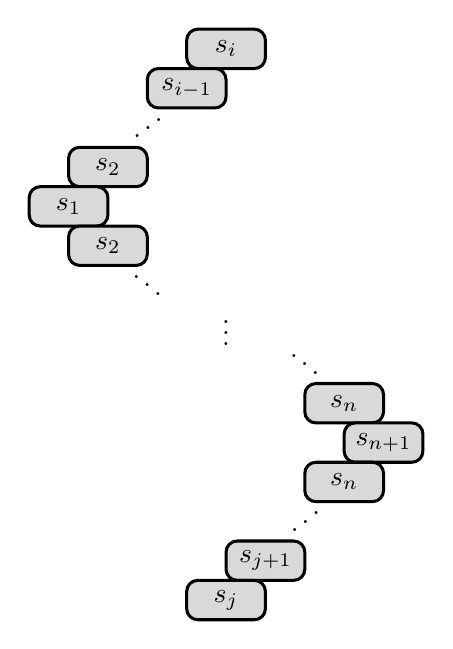
\begin{tikzpicture}[scale=0.5]
\heapblock{5}{15}{s_i};
\heapblock{4}{14}{s_{i-1}};
\draw (3,13.2) node {$\iddots$};
\heapblock{2}{12}{s_2};
\heapblock{1}{11}{s_1};
\heapblock{2}{10}{s_2};
\draw (3,9.2) node {$\ddots$};
\draw (5,8) node {$\vdots$};
\draw (7,7.2) node {$\ddots$};
\heapblock{8}{6}{s_n};
\heapblock{9}{5}{s_{n+1}};
\heapblock{8}{4}{s_{n}};
\draw (7,3.2) node {$\iddots$};
\heapblock{6}{2}{s_{j+1}};
\heapblock{5}{1}{s_{j}};
\end{tikzpicture}
\caption{Example of the heap for a type I element.}\label{fig:zigzag} 
\end{figure}

Note that there are an infinite number of type I elements and that every one of them is rigid, in the sense that each has a unique reduced expression.   The next proposition is~\cite[Proposition 3.1.3]{Ernst2010}.

\begin{proposition}\label{prop:zigzags}
If $w \in W(\C_{n})$ is of type I, then $w$ is FC with $n(w)=1$.  Conversely, if $n(w)=1$, then $w$ is of type I.  \qed
\end{proposition}

In order to define the type II elements, it will be helpful for us to define $\lambda=\lceil \frac{n-1}{2}\rceil$.  Then regardless of whether $n$ is odd or even, $2\lambda$ will always be the largest even number in $\{1,2,\dots,n+1\}$.  Similarly, $2\lambda+1$ will always be the largest odd number in $\{1,2,\dots, n+1\}$.

\begin{definition}
Define $\O=\{1,3, \dots, 2\lambda-1, 2\lambda+1\}$ and $\E=\{2, 4, \dots, 2\lambda-2, 2\lambda\}$.  Let $i$ and $j$ be of the same parity with $i<j$.  We define 
\[
\x_{i,j}=s_{i}s_{i+2}\cdots s_{j-2}s_{j}.
\]
Also, define
\[
\x_{\O}=\x_{1,2\lambda+1}=s_{1}s_{3}\cdots s_{2\lambda-1}s_{2\lambda+1},
\]
and
\[
\x_{\E}=\x_{2,2\lambda}=s_{2}s_{4}\cdots s_{2\lambda-2}s_{2\lambda}.
\]
If $w \in W(\C_n)$ is equal to a finite alternating product of $\x_{\O}$ and $\x_{\E}$, then we say that $w$ is of \emph{type II}.  (It is important to point out that the corresponding expressions are indeed reduced.)
\end{definition}

The following result is~\cite[Proposition 3.2.3]{Ernst2010}.

\begin{proposition}
If $w \in W(\C_{n})$ is of type II, then $w \in \FC(\C_{n})$ with $n(w)=\lambda$.   \qed
\end{proposition}

Note that if $w \in \FC(\C_{n})$, then $\lambda$ is the maximum value that $n(w)$ can take.  However, not every FC element with $n$-value $\lambda$ is of type II.  Furthermore, there are infinitely many type II elements.  

\end{subsection}

%%%%%%%  Non-cancellable elements %%%%%%%%%%%%%

\begin{subsection}{Weak star reductions and non-cancellable elements}\label{subsec:weak star}

The notion of a star operation was originally defined by Kazhdan and Lusztig in~\cite[\textsection 4.1]{Kazhdan1979} for simply-laced Coxeter systems (i.e., $m(s,t)\leq3$ for all $s,t \in S$) and was later generalized to arbitrary Coxeter systems in~\cite[\textsection 10.2]{Lusztig1985}.  If $I=\{s,t\}$ is a pair of noncommuting generators for $W$, then $I$ induces four partially defined maps from $W$ to itself, known as star operations. A star operation, when it is defined, respects the partition $W = \FC(W)\ \dot{\cup}\  (W \setminus \FC(W) )$ of the Coxeter group, and increases or decreases the length of the element to which it is applied by 1.  For our purposes, it is enough to define a weaker notion of a star operation that decreases length by 1, and so we will not develop the full generality.  

We now introduce the concept of weak star reducible, which is related to Fan's notion of cancellable in~\cite{Fan1997}.   Suppose $(W,S)$ is a Coxeter system of type $\Gamma$.  If $w \in \FC(\Gamma)$, then $w$ is \emph{left weak star reducible by $s$ with respect to $t$} to $sw$ if (i) $s\in \L(w)$, (ii) $t \in \L(sw)$ with $m(s,t) \geq 3$, and (iii) $tw \notin \FC(\Gamma)$.  Observe that condition (i) implies that $sw$ has length strictly smaller than $w$ while condition (iii) implies that $tw$ has length strictly larger than $w$.  We analogously define \emph{right weak star reducible by $s$ with respect to $t$}.  If $w$ is left (respectively, right) weak star reducible by $s$ with respect to $t$, then we define $\star^{L}_{s,t}(w)=sw$ (respectively, $\star^{R}_{s,t}(w)=ws$) and refer to $\star_{s,t}^{L}$ (respectively, $\star_{s,t}^{R}$) as a \emph{left} (respectively, \emph{right}) \emph{weak star reduction}.  If $w$ is either left or right weak star reducible by some $s\in S$, we say that $w$ is \emph{weak star reducible}.  Otherwise, we say that $w\in \FC(\Gamma)$ is \emph{non-cancellable}~\cite{Ernst2010}.  Note that the concept of weak star reducible is related to Fan's notion of cancellable in~\cite{Fan1997}.  

The non-cancellable elements of a Coxeter group $W$ are intimately related to the two-sided cells of the generalized Temperley--Lieb algebra (in the sense of Graham~\cite{Graham1995}) associated to $W$.  The connection between the non-cancellable elements and the two-sided cells has been examined for types $E$ and $\widetilde{A}$ in \cite{Fan1997} and \cite{Fan1999}, respectively.  Due to length considerations, we will not elaborate on the connection between the non-cancellable elements and the two-sided cells.

\begin{example}
Consider $w,w' \in \FC(\C_{n})$ having reduced expressions $\w=s_{1}s_{2}s_{1}$ and $\w'=s_{1}s_{2}$, respectively.  We see that $w$ is left (respectively, right) weak star reducible by $s_{1}$ with respect to $s_{2}$ to $s_2 s_1$ (respectively, $s_1 s_2$), and so $w$ is not non-cancellable.  However, $w'$ is non-cancellable.
\end{example}

If $w\in \FC(\Gamma)$ and $s \in \L(w)$ (respectively, $\R(w)$), it is clear that $sw$ (respectively, $ws$) is still FC.  This implies that if $w \in \FC(\Gamma)$ is left or right weak star reducible to $u$, then $u$ is also FC.

\begin{lemma}\label{lem:weak star ops preserve n-value}
Let $w \in \FC(\C_{n})$.  If $\star^{L}_{s,t}(w)$ (respectively, $\star^{R}_{s,t}(w)$) is defined, then $n(w)=n\left(\star^{L}_{s,t}(w)\right)$ (respectively, $n(w)=n\left(\star^{R}_{s,t}(w)\right)$).
\end{lemma}

\begin{proof}
This follows from Lemma~2.9 in~\cite{Shi2005} since weak star reductions (when defined) are a special case of ordinary star reductions.
\end{proof}

\begin{remark}\label{rem:wsrm properties}
If $w \in \FC(\C_{n})$, then $w$ is left weak star reducible by $s$ with respect to $t$ if and only if $w=stv$ (reduced) when $m(s,t)=3$, or $w=stsv$ (reduced) when $m(s,t)=4$.   Note that this characterization applies to $\FC(B_{n})$ and $\FC(B'_{n})$, as well.  In terms of heaps, if $\w=s_{x_1}\cdots s_{x_r}$ is a reduced expression for $w \in \FC(\C_{n})$, then $w$ is left weak star reducible by $s$ with respect to $t$ if and only if (i) there is an entry in $H(\w)$ labeled by $s$ that is not covered by any other entry, and (ii) the heap $H(t\w)$ contains one of the convex subheaps of Lemma~\ref{lem:impermissible heap configs}.  Of course, we have an analogous statement for right weak star reducible.
\end{remark}

The main results in~\cite{Ernst2010} are the classification of the non-cancellable elements in Coxeter groups of type $B$ and $\C$.

\begin{proposition}\label{prop:Bwsrm}
Let $w \in \FC(B_{n})$.  Then $w$ is non-cancellable if and only if $w$ is equal to either a product of commuting generators, $s_{1}s_{2}u$, or $s_{2}s_{1}u$, where $u$ is a product of commuting generators with $s_{1}, s_{2}, s_{3} \notin \supp(u)$.  We have an analogous statement for $\FC(B'_{n})$, where $s_{1}$ and $s_{2}$ are replaced with $s_{n+1}$ and $s_{n}$, respectively.
\end{proposition}

\begin{proof}
This is~\cite[Theorem 4.2.1]{Ernst2010}.
\end{proof}

\begin{proposition}\label{prop:affineCwsrm}
Let $w \in \FC(\C_{n})$.  Then $w$ is non-cancellable if and only if $w$ is equal to one of the elements on the following list.
\begin{enumerate}
\item \label{prop:affineCwsrm 1} $uv$, where $u$ is a type $B$ non-cancellable element and $v$ is a type $B'$ non-cancellable element with $\supp(u)\cap \supp(v)=\emptyset$;
\item \label{prop:affineCwsrm 2} $\z^{R,2k}_{1,1}$, $\z^{L,2k}_{n+1,n+1}$, $\z^{L,2k+1}_{n+1,1}$, and $\z^{R,2k+1}_{1,n+1}$; 
\item \label{prop:affineCwsrm 3} any type II element.
\end{enumerate}
\end{proposition}

\begin{proof}
This is~\cite[Theorem 5.1.1]{Ernst2010}.
\end{proof}

The elements listed in (\ref{prop:affineCwsrm 1}) of Proposition~\ref{prop:affineCwsrm} include all possible products of commuting generators.  This includes $\x_{\O}$ and $\x_{\E}$, which are also included in (\ref{prop:affineCwsrm 3}).  The elements listed in (\ref{prop:affineCwsrm 2}) are the type I elements having left and right descent sets equal to one of the end generators.

\end{subsection}

%%%%%%%%%  Preparatory lemmas %%%%%%%%%%

\begin{subsection}{Preparatory lemmas}\label{subsec:prep lemmas}

Before proceeding, we make a comment on notation.  When representing convex subheaps of $H(w)$ for $w\in \FC(\C_n)$, we will use a \begin{tabular}{c} 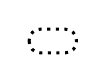
\begin{tikzpicture}[scale=0.3] \heapblank{0}{0}; \end{tikzpicture} \end{tabular} to indicate the absence of an entry in this location in any representation of $H(w)$.  It is important to note that the occurrence of a \begin{tabular}{c} 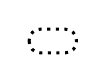
\begin{tikzpicture}[scale=0.3] \heapblank{0}{0}; \end{tikzpicture} \end{tabular} implies that an entry from the canonical representation of $H(w)$ cannot be shifted vertically from above or below to occupy the location of the \begin{tabular}{c} 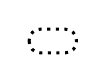
\begin{tikzpicture}[scale=0.3] \heapblank{0}{0}; \end{tikzpicture} \end{tabular}.

We will make frequent use of the following lemma, which allows us to determine whether an element is of type I.

\begin{lemma}\label{lem:zigzag}
Let $w \in \FC(\C_{n})$.  Suppose that $w$ has a reduced expression having one of the following FC elements as a subword:  
\begin{enumerate}
\item $\z^{L,2}_{2,n}=s_{2}s_{1}s_{2}s_{3} \cdots s_{n-1}s_{n}s_{n+1}s_{n}$,
\item $\z^{R,2}_{n,2}=s_{n}s_{n+1}s_{n}s_{n-1}\cdots s_{3}s_{2}s_{1}s_{2}$,
\item $\z^{R,2}_{1,1}=s_{1}s_{2}\cdots s_{n}s_{n+1}s_{n}\cdots s_{2}s_{1}$,
\item $\z^{L,2}_{n+1,n+1}=s_{n+1}s_{n}\cdots s_{2}s_{1}s_{2}\cdots s_{n}s_{n+1}$ .
\end{enumerate}
Then $w$ is of type I.
\end{lemma}

\begin{proof}
This is~\cite[Lemma 5.2.1]{Ernst2010}.
\end{proof}

The purpose of the next three lemmas (Lemmas \ref{lem:all filled in}, \ref{lem:zigzag subword}, and \ref{lem:typeI or nothing above}) is to prove Lemma~\ref{lem:main zigzag lemma}, which plays a crucial role in Section~\ref{sec:main results}.

\begin{lemma}\label{lem:all filled in}
Let $w \in \FC(\C_{n})$.  If the heap in Figure~\ref{fig:all filled in 1} is a saturated subheap of $H(w)$, where $i \neq n+1$, then the heap in Figure~\ref{fig:all filled in 2} is a convex subheap of $H(w)$, where every possible entry occurs in the region between the two occurrences of $s_1$ in Figure~\ref{fig:all filled in 1}.
\end{lemma}

\begin{figure}[!ht]
\subcaptionbox{\label{fig:all filled in 1}}[.3\textwidth]{
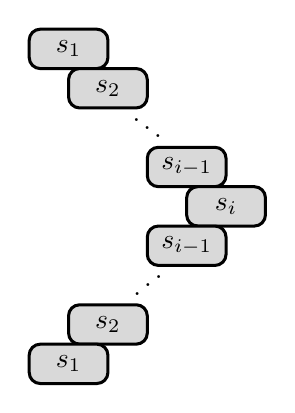
\begin{tikzpicture}[scale=0.5]
\heapblock{1}{9}{s_1};
\heapblock{2}{8}{s_2};
\draw (3,7.2) node {$\ddots$};
\heapblock{4}{6}{s_{i-1}};
\heapblock{5}{5}{s_i};
\heapblock{4}{4}{s_{i-1}};
\draw (3,3.2) node {$\iddots$};
\heapblock{2}{2}{s_2};
\heapblock{1}{1}{s_1};
\end{tikzpicture}
}
\subcaptionbox{\label{fig:all filled in 2}}[.3\textwidth]{
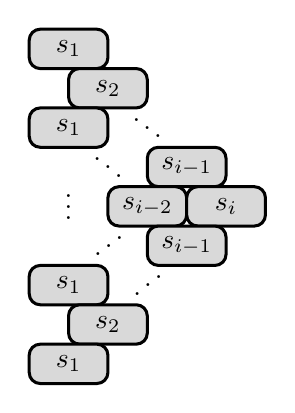
\begin{tikzpicture}[scale=0.5]
\heapblock{1}{9}{s_1};
\heapblock{2}{8}{s_2};
\heapblock{1}{7}{s_1};
\draw (2,6.2) node {$\ddots$};
\draw (3,7.2) node {$\ddots$};
\draw (1,5.2) node {$\vdots$};
\heapblock{4}{6}{s_{i-1}};
\heapblock{3}{5}{s_{i-2}};
\heapblock{5}{5}{s_i};
\heapblock{4}{4}{s_{i-1}};
\draw (2,4.2) node {$\iddots$};
\draw (3,3.2) node {$\iddots$};
\heapblock{1}{3}{s_1};
\heapblock{2}{2}{s_2};
\heapblock{1}{1}{s_1};
\end{tikzpicture}
}
\caption{Subheaps corresponding to Lemma~\ref{lem:all filled in}.}\label{fig:all filled in}
\end{figure}

\begin{proof}
This follows quickly from Lemma~\ref{lem:impermissible heap configs}; all other configurations will violate $w$ being FC.
\end{proof}

\begin{lemma}\label{lem:zigzag subword}
Let $w \in \FC(\C_{n})$.  Suppose there exists $i$ with $1<i < n+1$ such that $H(w)$ has two consecutive occurrences of entries labeled by $s_{i}$ such that there is no entry labeled by $s_{i+1}$ occurring between them.  Then the heap in Figure~\ref{fig:zigzag subword 1} is a convex subheap of $H(w)$.
\end{lemma}

\begin{proof}
We proceed by induction on $i$.  For the base case, let $i=2$ and suppose that there exist two consecutive occurrences of $s_{2}$ such that $s_{3}$ does not occur between them.  Then the heap in Figure~\ref{fig:zigzag subword 2} must be a convex subheap of $H(w)$, which implies that $s_{2}s_{1}s_{2}$ is a subword of $w$, as desired.  For the inductive step, assume that for $2\leq j \leq i-1$, whenever the hypotheses are met for $j$, $\z_{j,j}^{L,1}$ is a subword of $w$.  Now, assume that hypotheses are true for $i$.  Consider the entries in $H(w)$ corresponding to the two consecutive occurrences of $s_{i}$.  Since there is no entry labeled by $s_{i+1}$ occurring between these entries and $w$ is FC, there must be at least two entries labeled by $s_{i-1}$ occurring between the consecutive occurrences of $s_{i}$.  For sake of a contradiction, assume that there are three or more entries in $H(w)$ labeled by $s_{i-1}$ occurring between the minimal pair of entries labeled by $s_{i}$.  By induction (on $i-1$), the heap in Figure~\ref{fig:zigzag subword 3} is a saturated subheap of $H(w)$.  But by Lemma~\ref{lem:all filled in}, the convex closure of the saturated subheap occurring between the top two occurrences of $s_{1}$ must be completely filled in.  This produces a convex chain that corresponds to the subword $s_{2}s_{1}s_{2}s_{1}$, which contradicts $w \in \FC(\C_{n})$.  Therefore, between the consecutive occurrences of entries labeled by $s_{i}$, there must be exactly two occurrences of an entry labeled by $s_{i-1}$.  That is, by induction, the heap in Figure~\ref{fig:zigzag subword 1} is a convex subheap of $H(w)$ (and hence $\z_{i,i}^{L,1}$ is a subword of some reduced expression for $w$).
\end{proof}

\begin{figure}[!ht]
\subcaptionbox{\label{fig:zigzag subword 1}}[.3\textwidth]{
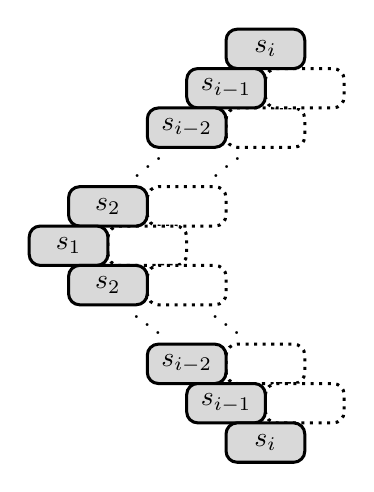
\begin{tikzpicture}[scale=0.5]
\heapblank{6}{9}
\heapblank{4}{7}
\heapblank{3}{6}
\heapblank{4}{5}
\heapblank{6}{3}
\heapblank{7}{2}
\heapblank{7}{10}
\draw (5,8.2) node {$\iddots$};
\draw (5,4.2) node {$\ddots$};
\heapblock{6}{11}{s_{i}};
\heapblock{5}{10}{s_{i-1}};
\heapblock{4}{9}{s_{i-2}};
\draw (3,8.2) node {$\iddots$};
\heapblock{2}{7}{s_2};
\heapblock{1}{6}{s_1};
\heapblock{2}{5}{s_2};
\draw (3,4.2) node {$\ddots$};
\heapblock{4}{3}{s_{i-2}};
\heapblock{5}{2}{s_{i-1}};
\heapblock{6}{1}{s_{i}};
\end{tikzpicture}
}
\subcaptionbox{\label{fig:zigzag subword 2}}[.3\textwidth]{
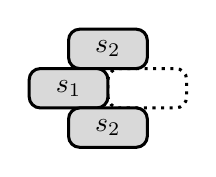
\begin{tikzpicture}[scale=0.5]
\heapblank{3}{2}
\heapblock{2}{3}{s_2};
\heapblock{1}{2}{s_1};
\heapblock{2}{1}{s_2};
\end{tikzpicture}
}
\subcaptionbox{\label{fig:zigzag subword 3}}[.3\textwidth]{
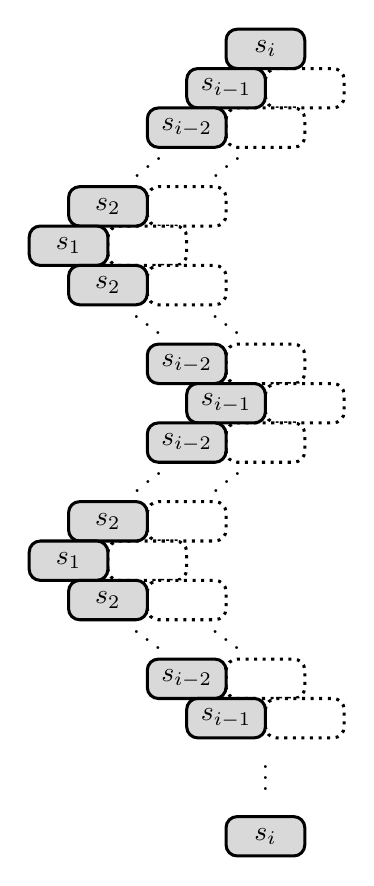
\begin{tikzpicture}[scale=0.5]
\heapblank{7}{18}
\heapblank{6}{17}
\heapblank{4}{15}
\heapblank{3}{14}
\heapblank{4}{13}
\heapblank{6}{11}
\draw (5,16.2) node {$\iddots$};
\draw (5,12.2) node {$\ddots$};
\heapblank{7}{10}
\heapblank{6}{9}
\heapblank{4}{7}
\heapblank{3}{6}
\heapblank{4}{5}
\heapblank{6}{3}
\heapblank{7}{2}
\draw (5,8.2) node {$\iddots$};
\draw (5,4.2) node {$\ddots$};
\heapblock{6}{19}{s_{i}};
\heapblock{5}{18}{s_{i-1}};
\heapblock{4}{17}{s_{i-2}};
\draw (3,16.2) node {$\iddots$};
\heapblock{2}{15}{s_2};
\heapblock{1}{14}{s_1};
\heapblock{2}{13}{s_2};
\draw (3,12.2) node {$\ddots$};
\heapblock{4}{11}{s_{i-2}};
\heapblock{5}{10}{s_{i-1}};
\heapblock{4}{9}{s_{i-2}};
\draw (3,8.2) node {$\iddots$};
\heapblock{2}{7}{s_2};
\heapblock{1}{6}{s_1};
\heapblock{2}{5}{s_2};
\draw (3,4.2) node {$\ddots$};
\heapblock{4}{3}{s_{i-2}};
\heapblock{5}{2}{s_{i-1}};
\draw (6,0.7) node {$\vdots$};
\heapblock{6}{-1}{s_{i}};
\end{tikzpicture}
}
\caption{Subheaps corresponding to Lemma~\ref{lem:zigzag subword}.}
\end{figure}

\begin{lemma}\label{lem:typeI or nothing above}
Let $w \in \FC(\C_{n})$ such that $s_{2}s_{1}s_{2}$ is a subword of some reduced expression for $w$ and let $i$ be the largest index such that the heap in Figure~\ref{fig:typeI or nothing above 1} is a saturated subheap of $H(w)$.  Then one or both of the following must be true about $w$:
\begin{enumerate}
\item $w$ is of type I; 
\item the subheap in Figure~\ref{fig:typeI or nothing above 2} is the northwest corner of $H(w)$.  In particular, the entry labeled by $s_{i}$ in Figure~\ref{fig:typeI or nothing above 2} is not covered.
\end{enumerate}
\end{lemma}

\begin{figure}[!ht]
\subcaptionbox{\label{fig:typeI or nothing above 1}}[.3\textwidth]{
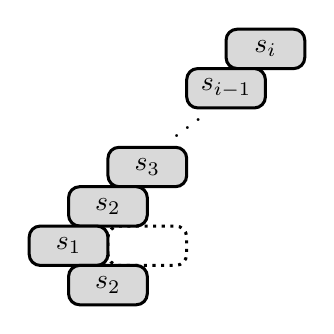
\begin{tikzpicture}[scale=0.5]
\heapblank{3}{2}
\heapblock{6}{7}{s_{i}};
\heapblock{5}{6}{s_{i-1}};
\draw (4,5.2) node {$\iddots$};
\heapblock{3}{4}{s_3};
\heapblock{2}{3}{s_2};
\heapblock{1}{2}{s_1};
\heapblock{2}{1}{s_2};
\end{tikzpicture}
}
\subcaptionbox{\label{fig:typeI or nothing above 2}}[.3\textwidth]{
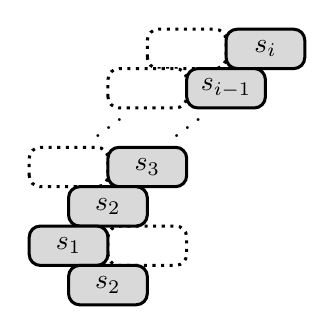
\begin{tikzpicture}[scale=0.5]
\heapblank{4}{7}
\heapblank{3}{6}
\heapblank{1}{4}
\draw (2,5.2) node {$\iddots$};
\heapblank{3}{2}
\heapblock{6}{7}{s_{i}};
\heapblock{5}{6}{s_{i-1}};
\draw (4,5.2) node {$\iddots$};
\heapblock{3}{4}{s_3};
\heapblock{2}{3}{s_2};
\heapblock{1}{2}{s_1};
\heapblock{2}{1}{s_2};
\end{tikzpicture}
}
\caption{Subheaps corresponding to Lemma~\ref{lem:typeI or nothing above}.}
\end{figure}

\begin{proof}
The higher entry labeled by $s_{2}$ cannot be covered by an entry labeled by $s_{1}$; otherwise, we produce one of the impermissible configurations of Lemma~\ref{lem:impermissible heap configs} and violate $w$ being FC.  Then the entry labeled by $s_{3}$ cannot be covered by an entry labeled by $s_{2}$; again, we would contradict Lemma~\ref{lem:impermissible heap configs}.  Iterating, we see that each entry on the diagonal of the subheap labeled by $s_{j}$, for $2 \leq j \leq i-1$, can only be covered by an entry labeled by $s_{j+1}$.  If $i<n+1$, we are done since the entry labeled by $s_{i}$ cannot be covered by an entry labeled by $s_{i-1}$.  Assume that $i=n+1$.  If the entry labeled by $s_{n+1}$ at the top of the diagonal in the subheap is covered by an entry labeled by $s_{n}$, then by Lemma~\ref{lem:zigzag}, $w$ is of type I.  If the entry labeled by $s_{n+1}$ is not covered, then we are done, as well.
\end{proof}

The previous lemma has versions corresponding to the southwest, northeast, and southeast corners of $H(w)$.  

As stated earlier, the purpose of the previous three lemmas was to aid in the proof of the next important lemma.  

\begin{lemma}\label{lem:main zigzag lemma}
Let $w \in \FC(\C_{n})$.  Suppose there exists $i$ with $1<i < n+1$ such that $H(w)$ has two consecutive occurrences of entries labeled by $s_{i}$ such that there is no entry labeled by $s_{i+1}$ occurring between them.  Then either $w$ is of type I or the heap in Figure~\ref{fig:main zigzag lemma 1} is a convex subheap of $H(w)$ and there are no other occurrences of entries labeled by $s_{1}, s_{2}, \dots, s_{i}$ in $H(w)$.
\end{lemma}

\begin{figure}[!ht]
\subcaptionbox{\label{fig:main zigzag lemma 1}}[.4\textwidth]{
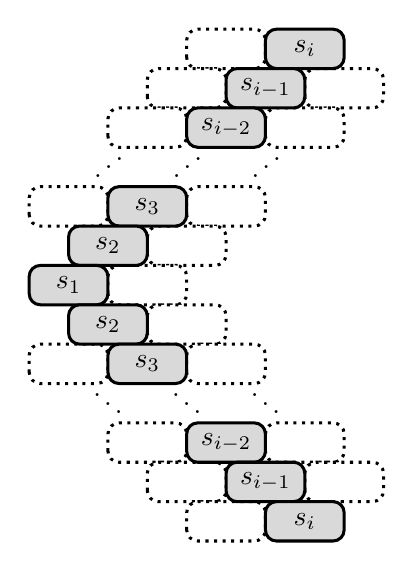
\begin{tikzpicture}[scale=0.5]
\heapblank{5}{13}
\heapblank{4}{12}
\heapblank{3}{11}
\draw (2,10.2) node {$\iddots$};
\heapblank{1}{9}
\heapblank{1}{5}
\draw (2,4.2) node {$\ddots$};
\heapblank{3}{3}
\heapblank{4}{2}
\heapblank{5}{1}
\heapblank{8}{12}
\heapblank{7}{11}
\draw (6,10.2) node {$\iddots$};
\heapblank{5}{9}
\heapblank{4}{8}
\heapblank{3}{7}
\heapblank{4}{6}
\heapblank{5}{5}
\draw (6,4.2) node {$\ddots$};
\heapblank{7}{3}
\heapblank{8}{2}
\heapblock{7}{13}{s_{i}};
\heapblock{6}{12}{s_{i-1}};
\heapblock{5}{11}{s_{i-2}};
\draw (4,10.2) node {$\iddots$};
\heapblock{3}{9}{s_3};
\heapblock{2}{8}{s_2};
\heapblock{1}{7}{s_1};
\heapblock{2}{6}{s_2};
\heapblock{3}{5}{s_3};
\draw (4,4.2) node {$\ddots$};
\heapblock{5}{3}{s_{i-2}};
\heapblock{6}{2}{s_{i-1}};
\heapblock{7}{1}{s_{i}};
\end{tikzpicture}
}
\subcaptionbox{\label{fig:main zigzag lemma 2}}[.4\textwidth]{
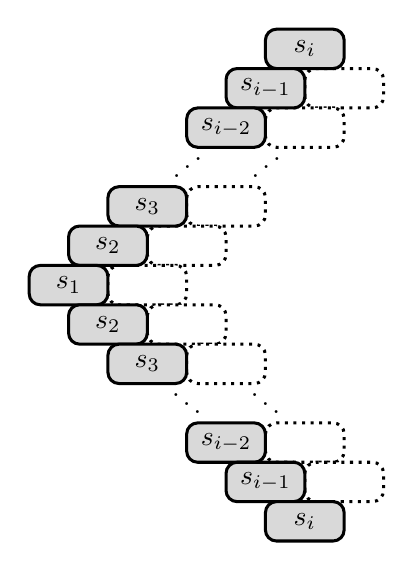
\begin{tikzpicture}[scale=0.5]
\heapblank{8}{12}
\heapblank{7}{11}
\draw (6,10.2) node {$\iddots$};
\heapblank{5}{9}
\heapblank{4}{8}
\heapblank{3}{7}
\heapblank{4}{6}
\heapblank{5}{5}
\draw (6,4.2) node {$\ddots$};
\heapblank{7}{3}
\heapblank{8}{2}
\heapblock{7}{13}{s_{i}};
\heapblock{6}{12}{s_{i-1}};
\heapblock{5}{11}{s_{i-2}};
\draw (4,10.2) node {$\iddots$};
\heapblock{3}{9}{s_3};
\heapblock{2}{8}{s_2};
\heapblock{1}{7}{s_1};
\heapblock{2}{6}{s_2};
\heapblock{3}{5}{s_3};
\draw (4,4.2) node {$\ddots$};
\heapblock{5}{3}{s_{i-2}};
\heapblock{6}{2}{s_{i-1}};
\heapblock{7}{1}{s_{i}};
\end{tikzpicture}
}\\
\vspace{1em}
\subcaptionbox{\label{fig:main zigzag lemma 3}}[.4\textwidth]{
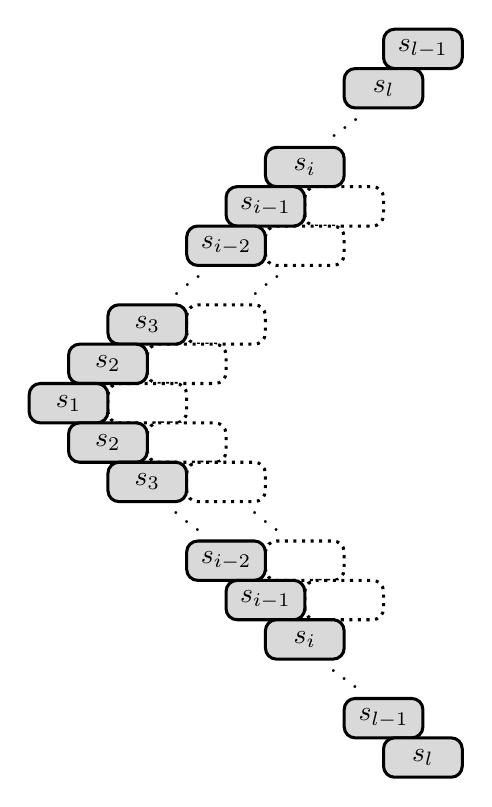
\begin{tikzpicture}[scale=0.5]
\heapblank{8}{12}
\heapblank{7}{11}
\draw (6,10.2) node {$\iddots$};
\heapblank{5}{9}
\heapblank{4}{8}
\heapblank{3}{7}
\heapblank{4}{6}
\heapblank{5}{5}
\draw (6,4.2) node {$\ddots$};
\heapblank{7}{3}
\heapblank{8}{2}
\heapblock{10}{16}{s_{l-1}};
\heapblock{9}{15}{s_{l}};
\draw (8,14.2) node {$\iddots$};
\heapblock{7}{13}{s_{i}};
\heapblock{6}{12}{s_{i-1}};
\heapblock{5}{11}{s_{i-2}};
\draw (4,10.2) node {$\iddots$};
\heapblock{3}{9}{s_3};
\heapblock{2}{8}{s_2};
\heapblock{1}{7}{s_1};
\heapblock{2}{6}{s_2};
\heapblock{3}{5}{s_3};
\draw (4,4.2) node {$\ddots$};
\heapblock{5}{3}{s_{i-2}};
\heapblock{6}{2}{s_{i-1}};
\heapblock{7}{1}{s_{i}};
\draw (8,0.2) node {$\ddots$};
\heapblock{9}{-1}{s_{l-1}};
\heapblock{10}{-2}{s_{l}};
\end{tikzpicture}
}
\subcaptionbox{\label{fig:main zigzag lemma 4}}[.4\textwidth]{
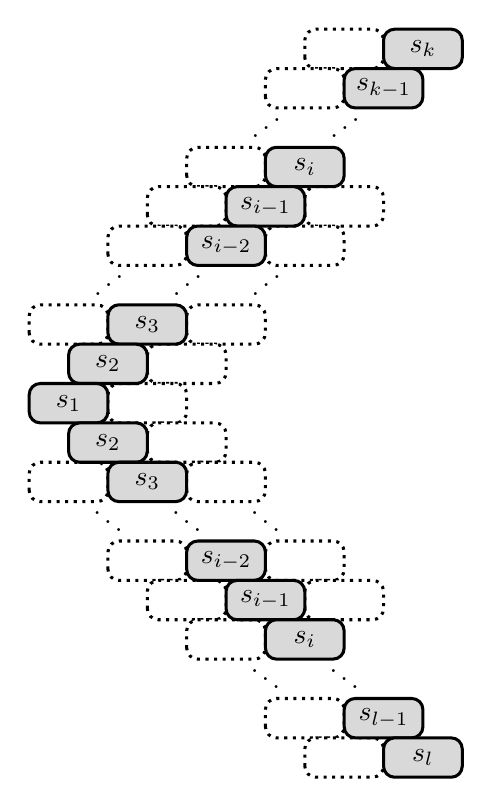
\begin{tikzpicture}[scale=0.5]
\heapblank{8}{16}
\heapblank{7}{15}
\draw (6,14.2) node {$\iddots$};
\heapblank{5}{13}
\heapblank{4}{12}
\heapblank{3}{11}
\draw (2,10.2) node {$\iddots$};
\heapblank{1}{9}
\heapblank{1}{5}
\draw (2,4.2) node {$\ddots$};
\heapblank{3}{3}
\heapblank{4}{2}
\heapblank{5}{1}
\heapblank{8}{12}
\heapblank{7}{11}
\draw (6,10.2) node {$\iddots$};
\heapblank{5}{9}
\heapblank{4}{8}
\heapblank{3}{7}
\heapblank{4}{6}
\heapblank{5}{5}
\draw (6,4.2) node {$\ddots$};
\heapblank{7}{3}
\heapblank{8}{2}
\draw (6,0.2) node {$\ddots$};
\heapblank{7}{-1}
\heapblank{8}{-2}
\heapblock{10}{16}{s_{k}};
\heapblock{9}{15}{s_{k-1}};
\draw (8,14.2) node {$\iddots$};
\heapblock{7}{13}{s_{i}};
\heapblock{6}{12}{s_{i-1}};
\heapblock{5}{11}{s_{i-2}};
\draw (4,10.2) node {$\iddots$};
\heapblock{3}{9}{s_3};
\heapblock{2}{8}{s_2};
\heapblock{1}{7}{s_1};
\heapblock{2}{6}{s_2};
\heapblock{3}{5}{s_3};
\draw (4,4.2) node {$\ddots$};
\heapblock{5}{3}{s_{i-2}};
\heapblock{6}{2}{s_{i-1}};
\heapblock{7}{1}{s_{i}};
\draw (8,0.2) node {$\ddots$};
\heapblock{9}{-1}{s_{l-1}};
\heapblock{10}{-2}{s_{l}};
\end{tikzpicture}
}
\caption{Subheaps corresponding to Lemma~\ref{lem:main zigzag lemma}.}
\end{figure}

\begin{proof}
Choose the largest index $i$ with $1<i<n+1$ such that $s_{i+1}$ does not occur between two consecutive occurrences of $s_{i}$ in $w$.  By Lemma~\ref{lem:zigzag subword}, $\z_{i,i}^{L,1}$ is a subword of some reduced expression for $w$ and the heap in Figure~\ref{fig:main zigzag lemma 2} is a convex subheap of $H(w)$.  Let $k$ be largest index with $i\leq k \leq n+1$ such that each entry labeled by $s_{j}$ on the upper diagonal in the subheap of Figure~\ref{fig:main zigzag lemma 1} covers an entry labeled by $s_{j-1}$ for $j\leq k$.  Similarly, let $l$ be the largest index with $i\leq l \leq n+1$ such that each entry on the lower diagonal labeled by $s_{j}$ is covered by an entry labeled by $s_{j-1}$ for $j\leq l$.  Then the heap in Figure~\ref{fig:main zigzag lemma 3} is a convex subheap of $H(w)$.  By the northwest and southwest versions of Lemma~\ref{lem:typeI or nothing above}, the heap in Figure~\ref{fig:main zigzag lemma 4} must be a convex subheap of $H(w)$.  If neither of $k$ or $l$ are equal to $n+1$, then we are done since the entry labeled by $s_{k}$ (respectively, $s_{l}$) cannot be covered by (respectively, cover) an entry labeled by $s_{k-1}$ (respectively, $s_{l-1}$); otherwise, we contradict $w \in \FC(\C_{n})$.  Assume that $k=n+1$; the case $l=n+1$ follows by a symmetric argument.  If the entry labeled by $s_{n+1}$ is covered, it must be covered by an entry labeled by $s_{n}$.  But by Lemma~\ref{lem:zigzag}, $w$ would then be of type I.
\end{proof}

Note that all of the previous lemmas of this section have analogous statements where $s_{1}$ and $s_{2}$ are replaced with $s_{n+1}$ and $s_{n}$, respectively.

\end{subsection}

\end{section}

%%%%%%%%%%% Generalized Temperley--Lieb algebras %%%%%%%%%%%%%

\begin{section}{Generalized Temperley--Lieb algebras}\label{sec:gen TL-algebras}

If $(W,S)$ is Coxeter system of type $\Gamma$, the associated Hecke algebra $\H(\Gamma)$ is an algebra with a basis given by $\{T_w\mid w \in W\}$ and relations that deform the relations of $W$ by a parameter $q$. In general, $\TL(\Gamma)$ is a quotient of $\H(\Gamma)$, having several bases indexed by the FC elements of $W$~\cite[Theorem 6.2]{Graham1995}.  Except for in the case of type $A$, there are many Temperley--Lieb type quotients that appear in the literature.  That is,  some authors define a Temperley--Lieb algebra to be a different quotient of $\H(\Gamma)$ than the one we are interested in.  In particular, the blob algebra of~\cite{Martin1994} is a smaller Temperley--Lieb type quotient of $\H(B_{n})$ than $\TL(B_{n})$.  Also, the symplectic blob algebra of~\cite{Green2012} and ~\cite{Martin2007} is a finite rank quotient of $\H(\C_{n})$, whereas, $\TL(\C_{n})$ is of infinite rank.  Furthermore, despite being infinite dimensional, the two-boundary Temperley--Lieb algebra of~\cite{Gier2009} is a different quotient of $\H(\C_n)$ than $\TL(\C_{n})$.  Typically, authors that study these usually smaller Temperley--Lieb type quotients are interested in representation theory, whereas our motivation is Kazhdan--Lusztig theory.

%%%%%%%%%%% Hecke algebra %%%%%%%%%%%%%

\begin{subsection}{Hecke algebras}

Let $\Gamma$ be an arbitrary Coxeter graph.  We define the \emph{Hecke algebra} of type $\Gamma$, denoted by $\H_{q}(\Gamma)$, to be the $\Z[q,q^{-1}]$-algebra with basis consisting of elements $T_{w}$, for all $w \in W(\Gamma)$, satisfying
\[
T_{s}T_{w}=\begin{cases}
T_{sw},  & \text{if } \ell(sw)>\ell(w), \\
qT_{sw}+(q-1)T_{w},  & \text{if } \ell(sw)<\ell(w)
\end{cases}
\]
where $s \in S(\Gamma)$ and $w \in W(\Gamma)$.  This is enough to compute $T_{x}T_{w}$ for arbitrary $x, w \in W(\Gamma)$.  Also, it follows from the definition that each $T_{w}$ is invertible.  It is convenient to extend the scalars of $\H_{q}(\Gamma)$ to produce an $\A$-algebra, $\H(\Gamma)=\A \otimes_{\Z[q,q^{-1}]} \H_{q}(\Gamma)$, where $\A=\Z[v,v^{-1}]$ and $v^{2}=q$.  The Laurent polynomial $v+v^{-1} \in \A$ occurs frequently and will be denoted by $\delta$.  

Since $W(\C_{n})$ is an infinite group, $\H(\C_{n})$ is an $\A$-algebra of infinite rank.  On the other hand, since $W(B_{n})$ and $W(B'_{n})$ are finite, both $\H(B_{n})$ and $\H(B'_{n})$ are of finite rank.

For more on Hecke algebras, we refer the reader to~\cite[Chapter 7]{Humphreys1990}.

\end{subsection}

%%%%%%%%%%%%% Temperley--Lieb algebras %%%%%%%%%%%%

\begin{subsection}{Temperley--Lieb algebras}\label{subsec:TL-algebras}

Let $J(\Gamma)$ be the two-sided ideal of $\H(\Gamma)$ generated by the set $\{J_{s,t}\mid 3\leq m(s,t)<\infty\}$, where
\[
J_{s,t}=\sum_{w \in \langle s, t \rangle}T_{w}
\]
and $\langle s, t \rangle$ is the subgroup generated by $s$ and $t$.

Following Graham~\cite[Definition 6.1]{Graham1995}, we define the \emph{(generalized) Temperley--Lieb algebra}, $\TL(\Gamma)$, to be the quotient $\A$-algebra $\H(\Gamma)/J(\Gamma)$.  We denote the corresponding canonical epimorphism by $\phi: \H(\Gamma) \to \TL(\Gamma)$.  Let $t_{w}=\phi(T_{w})$.  The following fact is due to Graham~\cite[Theorem 6.2]{Graham1995}.

\begin{theorem}\label{t-basis}
The set $\{t_{w}\mid w \in \FC(\Gamma)\}$ is an $\A$-basis for $\TL(\Gamma)$. \qed
\end{theorem}

We will refer to the basis of Theorem~\ref{t-basis} as the \emph{$t$-basis}.  For our purposes, it will be more useful to work a different basis, which we define in terms of the $t$-basis.

\begin{definition}
For each $s \in S(\Gamma)$, define $b_{s}=v^{-1}t_{s}+v^{-1}t_{e}$, where $e$ is the identity in $W(\Gamma)$.  If $s=s_{i}$, we will write $b_{i}$ in place of $b_{s_{i}}$.  If $w \in \FC(\Gamma)$ has reduced expression $\w=s_{x_{1}}\cdots s_{x_{r}}$, then we define 
\[
b_{\w}=b_{x_{1}}\cdots b_{x_{r}}.
\]
\end{definition}

Note that if $\w$ and $\w'$ are two different reduced expressions for $w \in \FC(\Gamma)$, then $b_{\w}=b_{\w'}$ since $\w$ and $\w'$ are commutation equivalent and $b_{i}b_{j}=b_{j}b_{i}$ when $m(s_{i}, s_{j})=2$.  So, we will write $b_{w}$ if we do not have a particular reduced expression in mind.  It is well known (and follows from~\cite[Proposition 2.4]{Green2006a}) that the set $\{b_{w}\mid w \in \FC(\Gamma)\}$ forms an $\A$-basis for $\TL(\Gamma)$.  This basis is referred to as the \emph{monomial basis} (or \emph{$b$-basis}).  We let $b_{e}$ denote the identity of $\TL(\Gamma)$.

Recall that $W(\C_{n})$ contains an infinite number of FC elements, while $W(B_{n})$ and $W(B'_{n})$ contain finitely many.  Hence $\TL(\C_{n})$ is an $\A$-algebra of infinite rank while $\TL(B_{n})$ and $\TL(B'_{n})$ are of finite rank.  (Note that we can have $\H(\Gamma)$ being of infinite rank while $\TL(\Gamma)$ is of finite rank.  In particular, $\TL(E_n)$ for $n\geq 9$ is finite dimensional while $\H(E_n)$ is of infinite rank.)

\end{subsection}

%%%%%%%%%%  A presentation for $\TL(\C)$ %%%%%%%%%%%%%

\begin{subsection}{A presentation for Temperley--Lieb algebras of type affine $C$}

It will be convenient for us to have a presentation for $\TL(\Gamma)$ in terms of generators and relations. The following theorem is special case of~\cite[Proposition 2.6]{Green2006a}.  

\begin{theorem}\label{thm:affine C relations}
The algebra $\TL(\C_{n})$ is generated (as a unital algebra) by $b_{1}, b_{2}, \dots, b_{n+1}$ with defining relations
\begin{enumerate}
\item $b_{i}^{2}=\delta b_{i}$ for all $i$;
\item $b_{i}b_{j}=b_{i}b_{j}$ if $|i-j|>1$;
\item $b_{i}b_{j}b_{i}=b_{i}$ if $|i-j|=1$ and $1< i,j < n+1$;
\item $b_{i}b_{j}b_{i}b_{j}=2b_{i}b_{j}$ if $\{i,j\}=\{1,2\}$ or $\{n,n+1\}$.
\end{enumerate}
In addition, $\TL(B_{n})$ (respectively, $\TL(B'_{n})$) is generated (as a unital algebra) by $b_{1}, b_{2}, \dots, b_{n}$ (respectively, $b_{2}, b_{3}, \dots, b_{n+1}$) with the corresponding relations above.  \hfill $\qed$
\end{theorem}

It is known that we can consider $\TL(B_{n})$ and $\TL(B'_{n})$ as subalgebras of $\TL(\C_{n})$ in the obvious way.

It will be useful for us to know what form an arbitrary product of monomial generators takes in $\TL(\C_{n})$.  The next lemma is similar to~\cite[Lemma 2.1.3]{Green2000}, which is a statement involving $W(B_{n})$.

\begin{lemma}\label{lem:powers of 2 and delta monomials}
Let $w \in \FC(\C_{n})$ and let $s \in S(\C_{n})$.  Then
\[
b_{s}b_{w}=2^{k}\delta^{m}b_{w'}
\]
for some $k, m \in \Z^{+}\cup \{0\}$ and $w' \in \FC(\C_{n})$.
\end{lemma}

\begin{proof}
We induct on the length of $w$.  For the base case, assume that $\ell(w)=0$ (i.e., $w=e$).  Then for any $s \in S(\C_{n})$, we have $b_{s}b_{e}=b_{s}$, which gives us our desired result.  Now, assume that $\ell(w)=p>1$.  There are three possibilities to consider.  

Case (1).  First, if $sw$ is reduced and FC, then $b_{s}b_{w}=b_{sw}$, which agrees with the statement of the lemma.

Case (2).  Second, if $sw$ is not reduced, then $s \in \L(w)$, and so we must be able to write $w=sv$ (reduced).  In this case, we see that $b_{s}b_{w}=b_{s}b_{s}b_{v}=\delta b_{s}b_{v}=\delta b_{w}$.  Again, this agrees with the statement of the lemma.

Case (3).  For the final case, assume that $sw$ is reduced, but not FC.  Then $sw$ must have a reduced expression containing the subword $sts$ if $m(s,t)=3$ or $stst$ if $m(s,t)=4$.  So, we must be able to write
\[
w=\begin{cases}
utsv, & \text{if } m(s,t)=3,\\
utstv, & \text{if } m(s,t)=4,
\end{cases}
\]
where each product is reduced, $u, v \in \FC(\C_{n})$, and $s$ commutes with every element of $\supp(u)$, so that
\[
sw=\begin{cases}
ustsv, & \text{if } m(s,t)=3,\\
uststv, & \text{if } m(s,t)=4.
\end{cases}
\]
This implies that
\[
b_{s}b_{w}=\begin{cases}
b_{u}b_{s}b_{t}b_{s}b_{v}=b_{u}b_{s}b_{v}, & \text{if } m(s,t)=3,\\
b_{u}b_{s}b_{t}b_{s}b_{t}b_{v}=2b_{u}b_{s}b_{t}b_{v}, & \text{if } m(s,t)=4.
\end{cases}
\]
Note that $\ell(u)+1+\ell(v) < p$ in the $m(s,t)=3$ case and that $\ell(u)+2+\ell(v) < p$ when $m(s,t)=4$.  So, we can apply the inductive hypothesis $\ell(u)+1$ (respectively, $\ell(u)+2$) times if $m(s,t)=3$ (respectively, $m(s,t)=4$) starting with $b_{s}b_{v}$ (respectively, $b_{t}b_{v}$).  Therefore, we obtain $b_{s}b_{w}=2^{k}\delta^{m}b_{w'}$ for some $k, m \in \Z^{+}\cup \{0\}$ and $w' \in \FC(\C_{n})$, as desired.
\end{proof}

If $b_{x_{1}}, b_{x_{2}}, \dots, b_{x_{p}}$ is any collection of $p$ monomial generators, then it follows immediately from Lemma~\ref{lem:powers of 2 and delta monomials}  that $b_{x_{1}}b_{x_{2}}\cdots b_{x_{p}}=2^{k}\delta^{m} b_{w}$ for some $k, m \in \Z^{+}\cup \{0\}$ and $w \in \FC(\C_{n})$.

\end{subsection}

%%%%%%%%%% Weak star reducibility and the monomial basis %%%%%%%%%%%%%

\begin{subsection}{Weak star reducibility and the monomial basis}

With respect to weak star reductions, computation involving monomial basis elements is ``well-behaved", as the next remark illustrates.

\begin{remark}\label{rem:monomial weak star reductions}
Suppose that $w \in \FC(\C_{n})$ is left weak star reducible by $s$ with respect to $t$.  Recall from Remark~\ref{rem:wsrm properties} that this implies that $w=stv$ (reduced) when $m(s,t)=3$ or $w=stsv$ (reduced) when $m(s,t)=4$.  In this case, we have
\[
b_{t}b_{w}=\begin{cases}
b_{tv},   & \text{if } m(s,t)=3, \\
2b_{tsv},   & \text{if } m(s,t)=4.
\end{cases}
\]
It is important to note that $\ell(tv)=\ell(w)-1$ when $m(s,t)=3$ and $\ell(tsv)=\ell(w)-1$ when $m(s,t)=4$.  We have a similar characterization for right weak star reducibility.  
\end{remark}

It is tempting to think that if $b_{w}$ is a monomial basis element such that $b_{t}b_{w}=2^{c}b_{y}$, where $c\in \{0,1\}$ and $\ell(y)<\ell(w)$, then $w$ is weak star reducible by some $s$ with respect to $t$, where $m(s,t)\geq 3$.  However, this is not true.  For example, let $w=s_{1}s_{2}s_{3}s_{4} \in \FC(\C_{n})$ with $n \geq 3$, so that $m(s_{2},s_{3})=3$, and let $t=s_{3}$.  Then
{\allowdisplaybreaks
\begin{align*}
b_{t}b_{w} &= b_{3}b_{1}b_{2}b_{3}b_{4} \\
&= b_{1}b_{3}b_{2}b_{3}b_{4}\\
&= b_{1}b_{3}b_{4} \\
&= b_{s_{1}s_{3}s_{4}}.
\end{align*}}%
We see that $\ell(s_{1}s_{3}s_{4}) < \ell(w)$, but $w$ is not left weak star reducible by $s_{3}$ (or any generator).  

The next lemma is useful for reversing the multiplication of monomials corresponding to weak star reductions.

\begin{lemma}\label{lem:weak star reverse}
Let $w \in \FC(\C_{n})$ and suppose that $w$ is left weak star reducible by $s$ with respect to $t$.  Then
\[
b_{s}b_{t}b_{w}=\begin{cases}
b_{w},   & \text{if } m(s,t)=3, \\
2b_{w},   & \text{if } m(s,t)=4.
\end{cases}
\]
We have an analogous statement if $w$ is right weak star reducible by $s$ with respect to $t$.
\end{lemma}

\begin{proof}
Suppose that $w$ is left weak star reducible by $s$ with respect to $t$.  Then we can write $w=stv$ (reduced) when $m(s,t)=3$ or $w=stsv$ (reduced) when $m(s,t)=4$, which implies that
\[
b_{t}b_{w}=\begin{cases}
b_{tv},   & \text{if } m(s,t)=3, \\
2b_{tsv},   & \text{if } m(s,t)=4.
\end{cases}
\]
Therefore, we have
{\allowdisplaybreaks
\begin{align*}
b_{s}b_{t}b_{w}=&\begin{cases}
b_{s}b_{tv},   & \text{if } m(s,t)=3, \\
2b_{s}b_{tsv},   & \text{if } m(s,t)=4,
\end{cases}\\
=& \begin{cases}
b_{stv},   & \text{if } m(s,t)=3, \\
2b_{stsv},   & \text{if } m(s,t)=4,
\end{cases}\\
=& \begin{cases}
b_{w},   & \text{if } m(s,t)=3, \\
2b_{w},   & \text{if } m(s,t)=4,
\end{cases}
\end{align*}}%
as desired.
\end{proof}

\end{subsection}

\end{section}

\end{document}